\documentclass{ximera}
\title{Series Tests}
\begin{abstract}
\end{abstract}

\usepackage{../Calc2_preamble}


\newcommand{\hh}{\hs{40pt}}

\newcommand{\ssm}{\vs{25pt}}
\newcommand{\sm}{\vs{75pt}}
\newcommand{\med}{\vs{150pt}}
\newcommand{\bg}{\vs{230pt}}

\newcommand{\dsum}{\displaystyle \sum}
\newcommand{\dsumone}{\dsum_{n=1}^{\infty}}




\newcommand{\du}{\; du}
\newcommand{\dv}{\; dv}
\newcommand{\dtheta}{\; d\theta}

%\newcommand{\sk}{\vs{20pt}
%\newcommand{\ssk}{\hs{10pt}


\begin{document}


\section{Introduction}
\begin{dialogue}
\item[Julia] There are so many tests to keep track of for series!
\item[Dylan] Did you say test?! When??? WHY HAS NO ONE TOLD ME?!
\item[James] Calm down Dylan! Julia was talking about \textit{series} tests, not an exam.
\item[Dylan] Oh, good, I was worried there for a second. Sucks how many series tests we have to keep track of, huh?
\item[Julia] Do you think you could help us out James? Maybe a trick to remember?
\item[James] Well, there's no better way to remember something than repetition!
\end{dialogue}
\section*{Strategies for Applying Series Tests} In Section 11.5, the text gives a very detailed description of when to try and apply each of our series tests. Here is a brief outline to follow when looking at a series $\sum a_n$:
	\begin{itemize}
		\item First thing to try: \textbf{the Divergence Test}. If $\dlim_{n \to \infty} a_n \neq 0$, then we know that the series $\sum a_n$ diverges and we are done right away! Otherwise, $\dlim_{n \to \infty} a_n = 0$ and we have to try an actual test.
		
		\item Next, try to see if the series is of a certain class that we know: a \textbf{Geometric Series}, a \textbf{$p$-series}, the Harmonic Series, etc.. Look for variations as well - if the series looks like a sum or difference of two geometric series, or a sum of a $p$-series and a geometric series, etc.. Remember, the sum or difference of two converging series converges (this is Theorem 1 in Sec. 11.2). (What happens if we add a diverging series with a converging series?)
		
		\item Identify if the series has all positive terms. If it does not, determine if it is an \textbf{Alternating Series} and try the \emph{Alternating Series Test}.
		
		\item If the series has negative terms and is not alternating or does not apply, you can try to determine if the series is \emph{absolutely convergent}, since absolute convergence implies convergence. Remember, this means determining whether $\sum |a_n|$ converges. You can either use the tests below for positive series, or use the \textbf{Ratio} or \textbf{Root Test}, as these are tests for absolute convergence. In particular, if there are any factorials involved, you likely want to use the \emph{ratio test}.
		
		\item Lastly for a non-positive series, make sure you have answered the question! Does it ask for \emph{absolute/conditional convergence}, or simply asks whether the series converges or diverges? If the former, make sure you fully investigate the series by checking for absolute convergence, especially if it is an alternating series.
		
		\item Now, if your series is positive, or you are examining $\sum |a_n|$, then we can apply the first three tests discussed in Sec. 11.3 - the \textbf{Direct \& Limit Comparison Tests} and the \textbf{Integral Test}. It's a good idea to try \emph{Direct comparison} first. If that fails due to the inequality going the wrong way, then use the \emph{Limit comparison test}.
		
		\item If all of the above has failed you, then we have the \emph{Integral Test} as our backup test. 
	\end{itemize}	
%\newpage

To help summarize the strategies you know, we will provide you this handy table.

\begin{image}
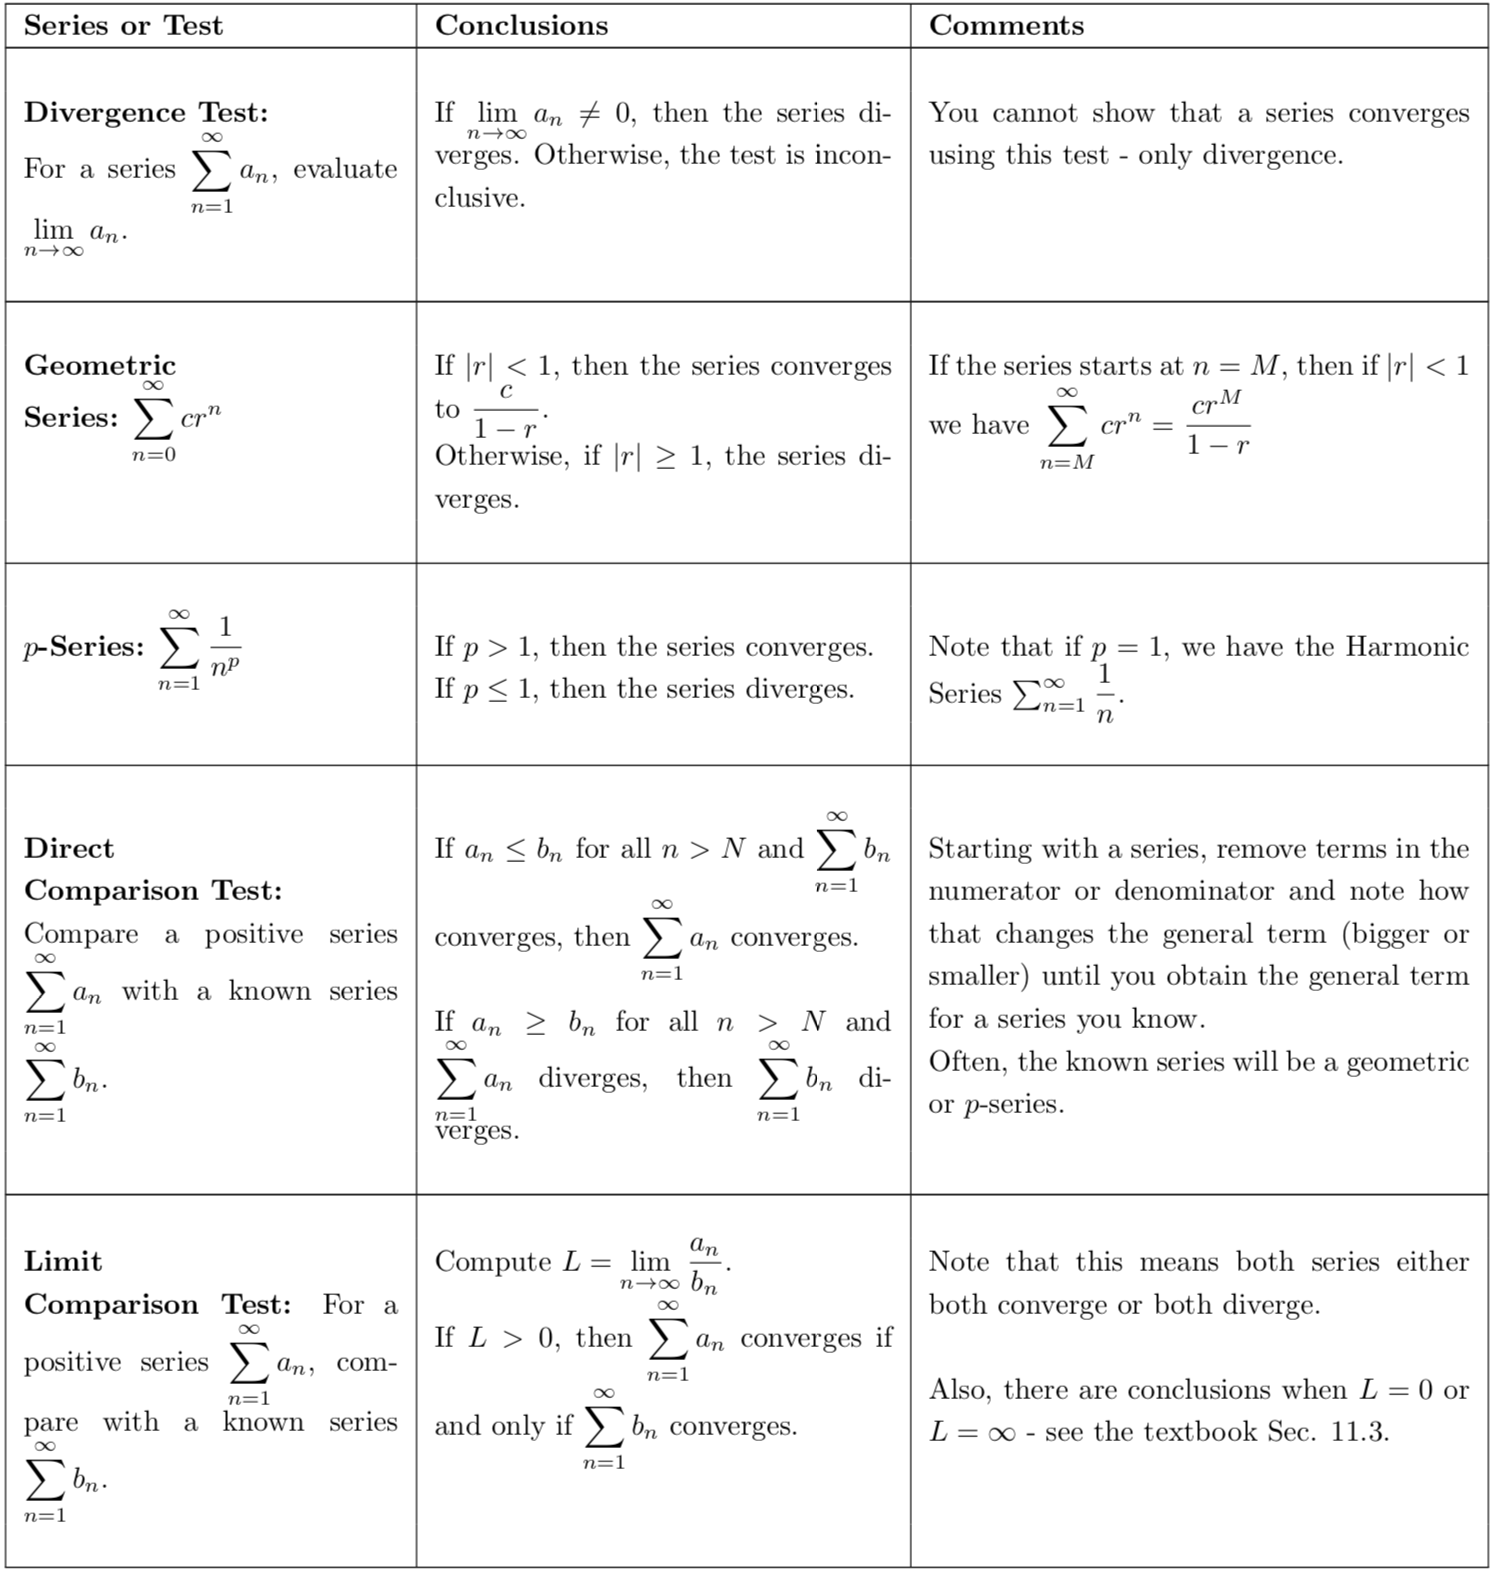
\includegraphics{Strat_Table1}
\end{image}
\begin{image}
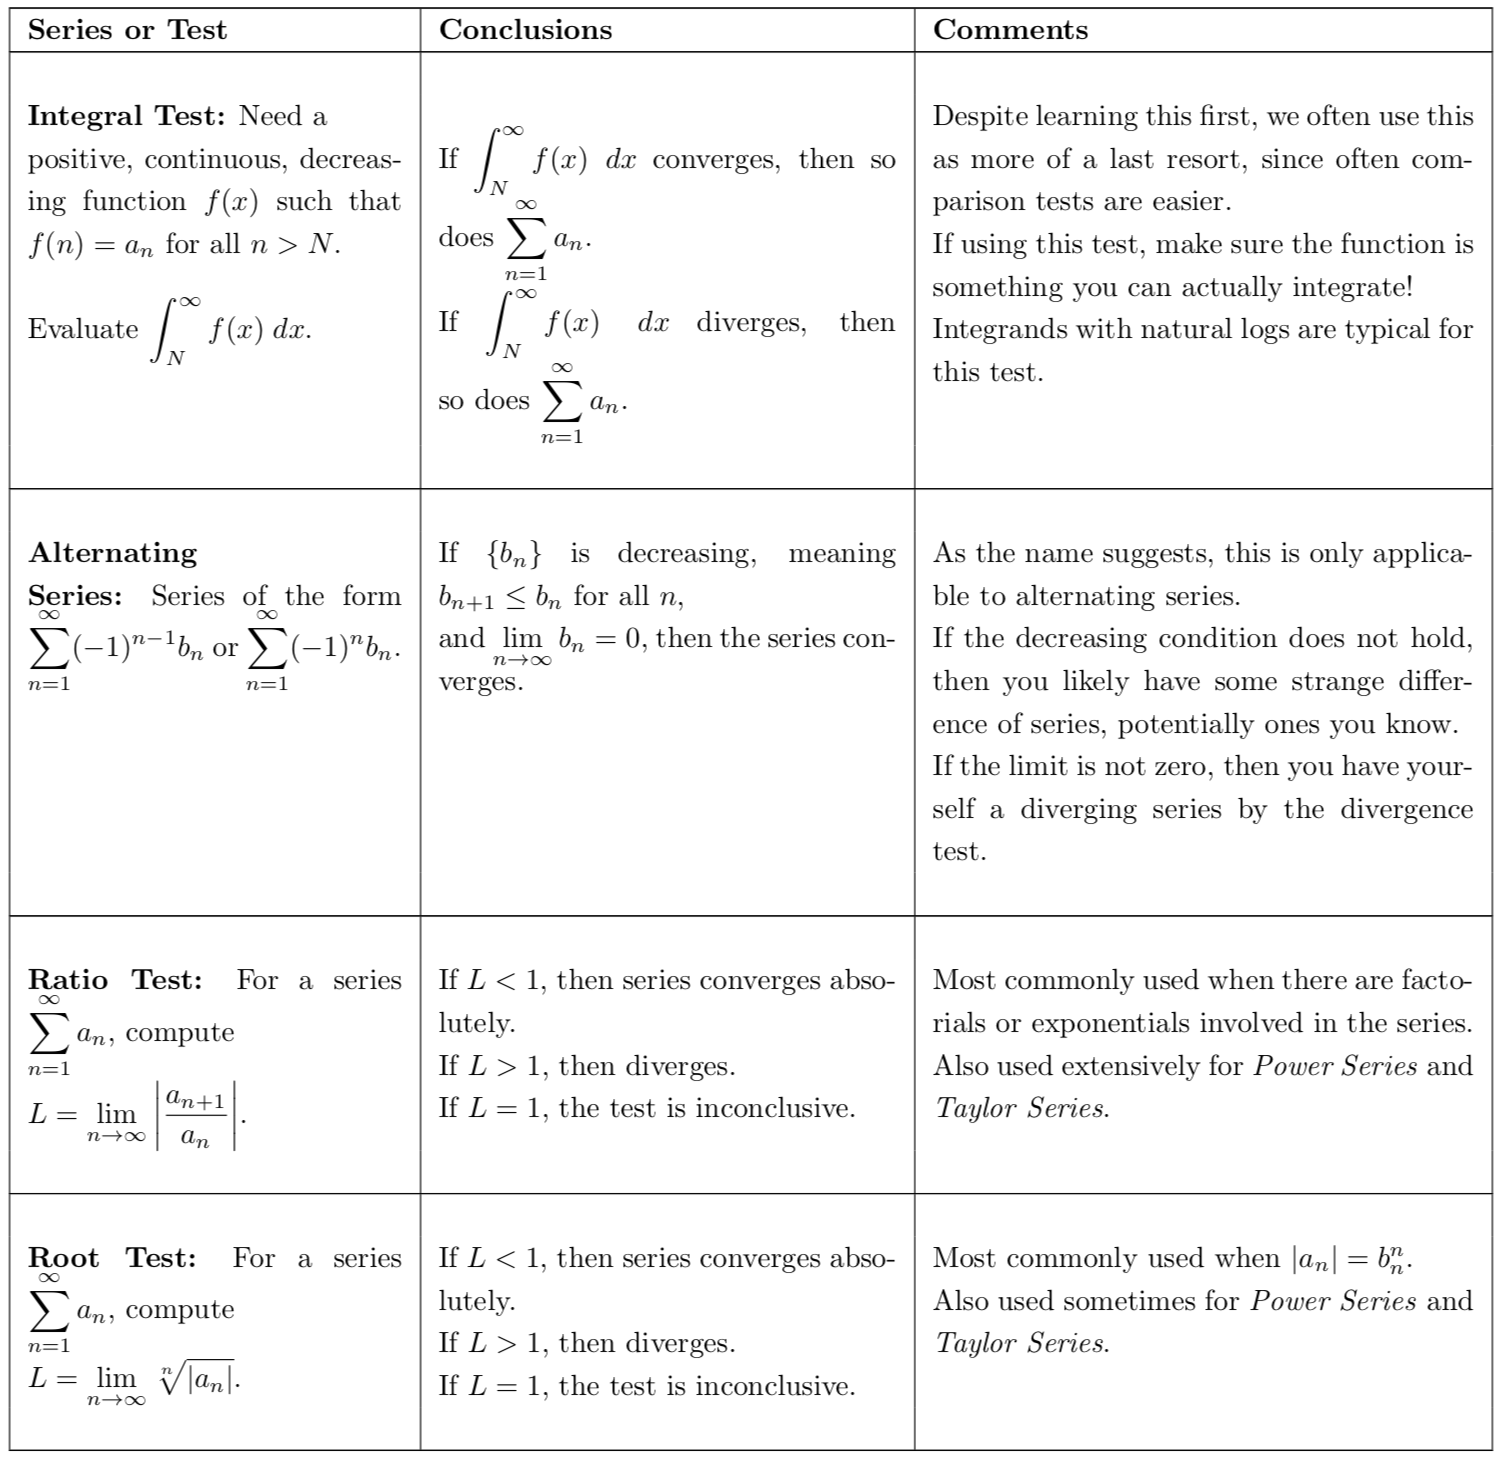
\includegraphics{Strat_Table2}
\end{image}

\newpage

\section*{Practice Problems} Try to utilize the tests above to determine if the given series is converging or diverging. If the series has negative terms, determine if the series is absolutely convergent, conditionally convergent, or divergent.

\begin{problem}
$\dsumone \df{n^2 + 2n}{n^3 + 3n^2 + 1}$
\begin{multipleChoice}
\choice[correct]{Diverges}
\choice{Conditionally Convergent}
\choice{Absolutely Convergent}
\end{multipleChoice}
\end{problem}
\begin{problem} $\dsumone \df{(-1)^{n+1}(3n+1)}{n!}$
\begin{multipleChoice}
\choice{Diverges}
\choice{Conditionally Convergent}
\choice[correct]{Absolutely Convergent}
\end{multipleChoice}
\end{problem}
\begin{problem} $\dsumone \df{e^n}{n^4}$
\begin{multipleChoice}
\choice[correct]{Diverges}
\choice{Conditionally Convergent}
\choice{Absolutely Convergent}
\end{multipleChoice}
\end{problem}
\begin{problem} $\dsumone \df{3^n}{(n+1)^n}$
\begin{multipleChoice}
\choice{Diverges}
\choice{Conditionally Convergent}
\choice[correct]{Absolutely Convergent}
\end{multipleChoice}
\end{problem}
\begin{problem}$\dsumone \df{2^n - 5^n}{7^n}$
\begin{multipleChoice}
\choice{Diverges}
\choice{Conditionally Convergent}
\choice[correct]{Absolutely Convergent}
\end{multipleChoice}
\end{problem}
\begin{problem} $\dsumone \df{\sin(n)}{n^2}$
\begin{multipleChoice}
\choice{Diverges}
\choice{Conditionally Convergent}
\choice[correct]{Absolutely Convergent}
\end{multipleChoice}
\end{problem}
\begin{problem}$\dsumone \df{1+(-1)^n}{n}$
\begin{multipleChoice}
\choice[correct]{Diverges}
\choice{Conditionally Convergent}
\choice{Absolutely Convergent}
\end{multipleChoice}
\end{problem}
\begin{problem} $\dsumone \df{n^n}{n!}$
\begin{multipleChoice}
\choice[correct]{Diverges}
\choice{Conditionally Convergent}
\choice{Absolutely Convergent}
\end{multipleChoice}
	\end{problem}
\begin{problem} $\dsumone \df{1}{n^{3/2} - (\ln(n))^4}$
\begin{multipleChoice}
\choice{Diverges}
\choice{Conditionally Convergent}
\choice[correct]{Absolutely Convergent}
\end{multipleChoice}
\end{problem}
\begin{problem} $\dsumone \df{1}{n+\sqrt{n}}$
\begin{multipleChoice}
\choice[correct]{Diverges}
\choice{Conditionally Convergent}
\choice{Absolutely Convergent}
\end{multipleChoice}
\end{problem}
\begin{problem} $\dsumone \df{\cos(\pi n)}{n^{2/3}}$
\begin{multipleChoice}
\choice{Diverges}
\choice[correct]{Conditionally Convergent}
\choice{Absolutely Convergent}
\end{multipleChoice}
\end{problem}
\begin{problem} $\dsumone \df{n^5}{5^n}$
\begin{multipleChoice}
\choice{Diverges}
\choice{Conditionally Convergent}
\choice[correct]{Absolutely Convergent}
\end{multipleChoice}
\end{problem}
\begin{problem} $\dsumone \df{(-1)^{n}}{\sqrt{n}(\ln(n))^2}$
\begin{multipleChoice}
\choice{Diverges}
\choice[correct]{Conditionally Convergent}
\choice{Absolutely Convergent}
\end{multipleChoice}
\end{problem}
\begin{problem} $\df{1}{2} - \df{1}{5} + \df{1}{4} - \df{1}{25} + \df{1}{8} - \df{1}{125} + \dots$
\begin{multipleChoice}
\choice{Diverges}
\choice[correct]{Conditionally Convergent}
\choice{Absolutely Convergent}
\end{multipleChoice}
\end{problem}

\end{document}